
\begin{figure}
  \centering 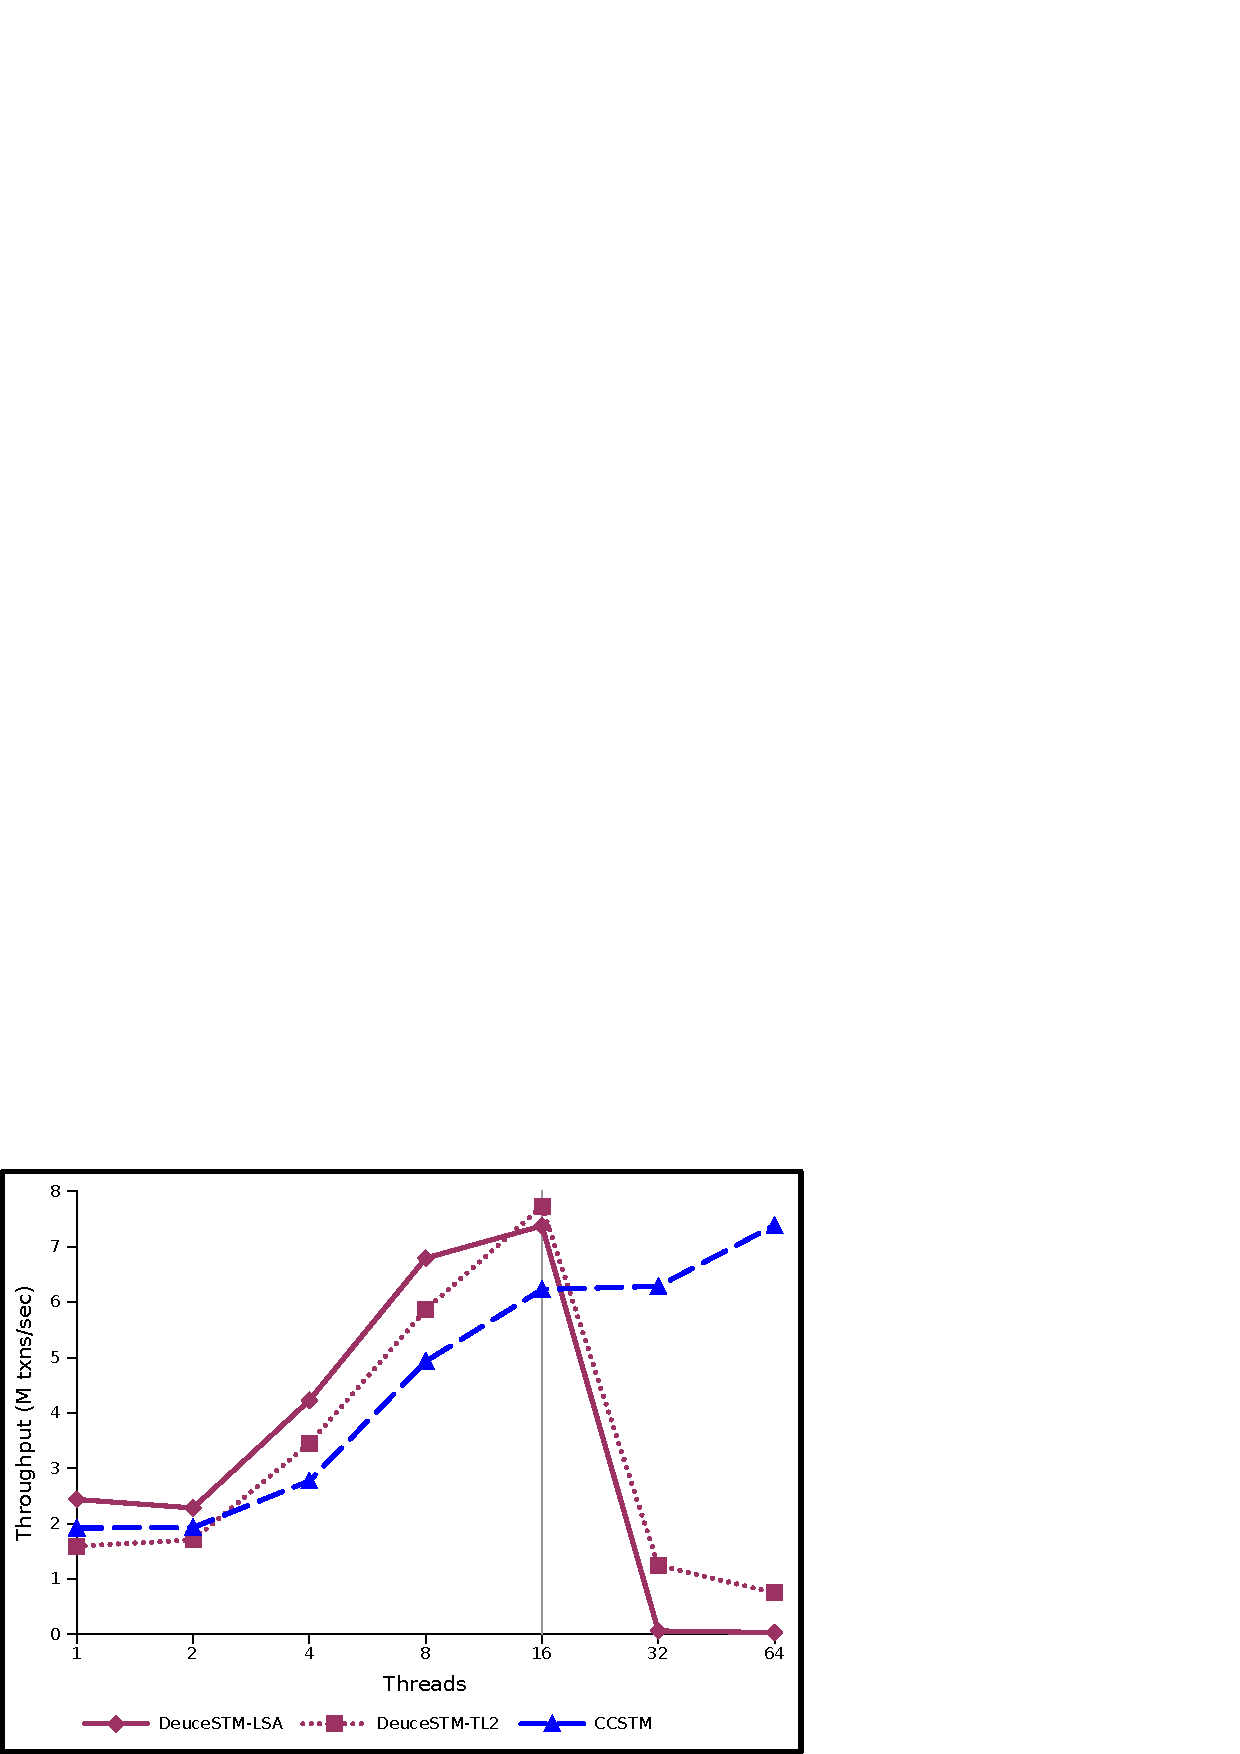
\includegraphics[clip=true,width=3in]{build/low_cont}

\caption{Throughput for the bank benchmark in a low contention scenario,
on a machine with 16 hardware thread contexts.  The number of accounts
is 64 times the number of threads.}

  \label{fig:lowcont}
\end{figure}

\begin{figure}
  \centering 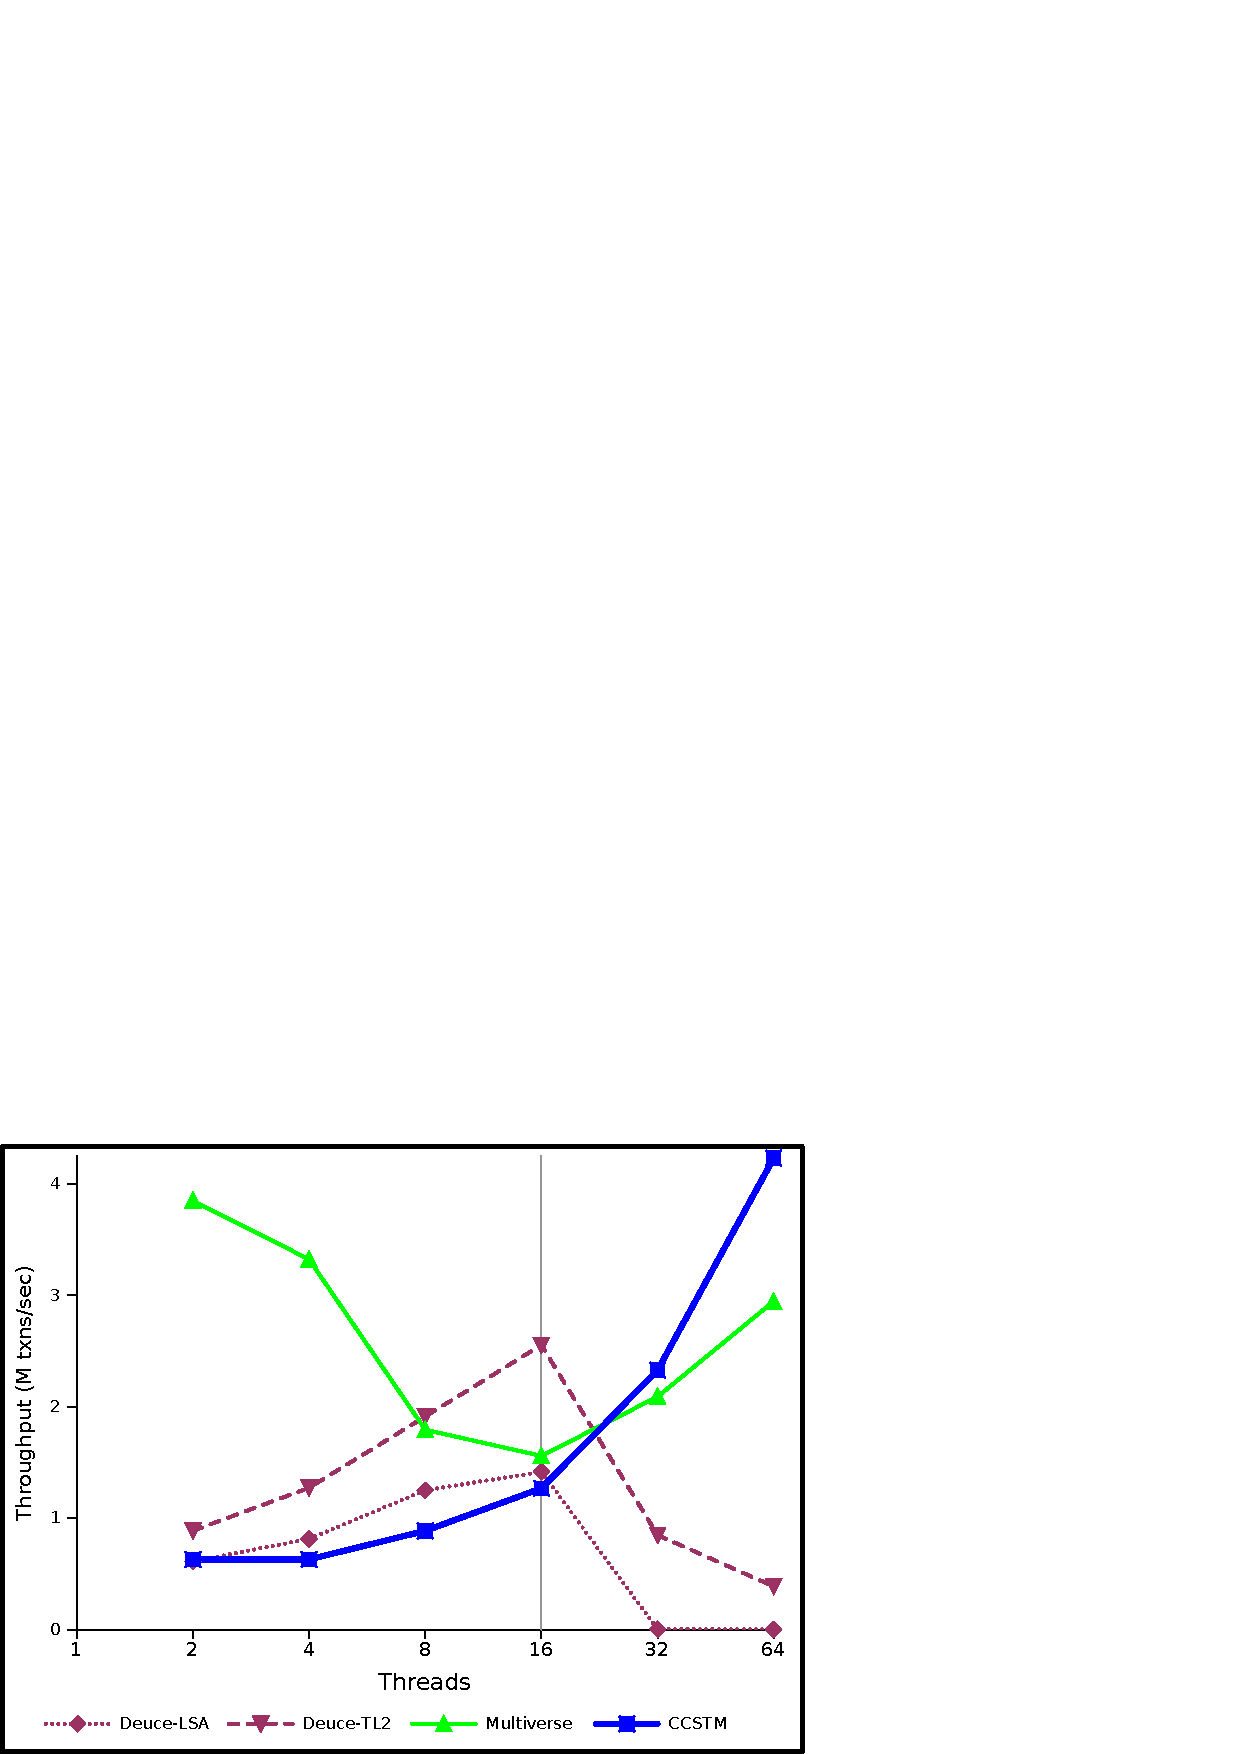
\includegraphics[clip=true,width=3in]{build/high_cont}

\caption{Throughput for a high contention scenario.  The number of accounts is
equal to the number of threads.  Each transaction touches two accounts.}

  \label{fig:highcont}
\end{figure}

CCSTM's implementation as an unprivileged library introduces several possible inefficiencies:
\type{Ref} adds a level of indirection;
JVM erasure adds boxing overheads for \xtype{Ref}{T} when \typeparam{T} is a
primitive type; dynamic scoping involves a hash table lookup, either implicitly
inside \type{ThreadLocal} or explicitly with a \type{Thread} key; low-level
atomic operations performed by the STM cannot use the unchecked primitives in
\code{sun.misc.Unsafe}; \todo{more}

must use \type{ThreadLocal} or a map keyed on
\type{Thread}, both of which add a hash table lookup , which is slower
than adding a field to the underlying thread instance.


To verify that CCSTM's library-based design does not impose a prohibitive
performance penalty, we compared it to Deuce STM and Multiverse, STMs for
the JVM that perform bytecode rewriting during class
loading~\cite{deucestm,multiverse}.

Experiments were run on a Dell Precision T7500n with two quad-core
2.66Ghz Intel Xeon X5550 processors, and 24GB of RAM.  Hyper-Threading was
enabled, yielding a total of 16 hardware thread contexts.  We used Scala
version 2.8.0.Beta1.  We ran our experiments in
Sun's Java~SE Runtime Environment, build 1.6.0\_16-b01, using the HotSpot
64-Bit Server VM.  Deuce STM was version 1.3.0.  Multiverse was version 0.4.
%We enabled dynamic escape analysis and compressed
%oops.

We performed a direct encoding of Deuce STM's bank benchmark into
Scala+CCSTM, and compared this version to the Java original running
under the bytecode rewriting STMs.  (While the example code in this paper uses an
immutable \type{Money} numeric type, the evaluated benchmark uses 32-bit
floating point values like the original.)  Deuce STM provides two algorithms,
TL2 and LSA.  In addition, it allows an optional contention manager to
be used.  For each run, we report the throughput of a Deuce STM algorithm
as the maximum of the throughput with or without contention management.
For almost all configurations we tested, contention management reduced
throughput.  CCSTM and Multiverse were tested using their default
configuration.

This benchmark includes its own harness, which we configured so
that no overdrafts were triggered.  We used a 4 second warmup, and
then measured the number of transactions committed during 10 seconds,
averaging across three invocations of the JVM.  For the low-contention
experiment (Figure~\ref{fig:lowcont}) we set the number of accounts
to 64 times the number of threads.  For the high-contention experiment
(Figure~\ref{fig:highcont}) we set the number of accounts to the number of
threads.  Single-threaded execution is not included in the high-contention
setup, as it has no contention.  Because at most 16 threads are executing
at any time, high-contention runs have fewer conflicts at 32 and 64
threads than for lower thread counts, and so can continue to scale.

\todo{talk about multiverse}
The TL2 version of Deuce STM is faster than CCSTM for both experiments when
the multi-threading level is less than or equal to one.  The difference
is largest for the high-contention scenario, where threads are often
obstructed.  Deuce STM does not block threads that cannot proceed, and it
does not even use sleeps or yields.  This strategy works well when every
thread gets its own hardware context, but results in a catastrophic
performance dropoff for higher thread counts.  CCSTM's synchronization
implementation is more expensive, but yields stable performance even at
high multi-threading levels.

Deuce STM and CCSTM have different algorithms and engineering tradeoffs,
so these experiments do not allow us to exactly measure the overhead
imposed by the library-only design.  They do demonstrate, however,
that any overhead that does exist is small enough to be tolerable.
